% Created by tikzDevice version 0.7.0 on 2014-07-29 02:50:00
% !TEX encoding = UTF-8 Unicode
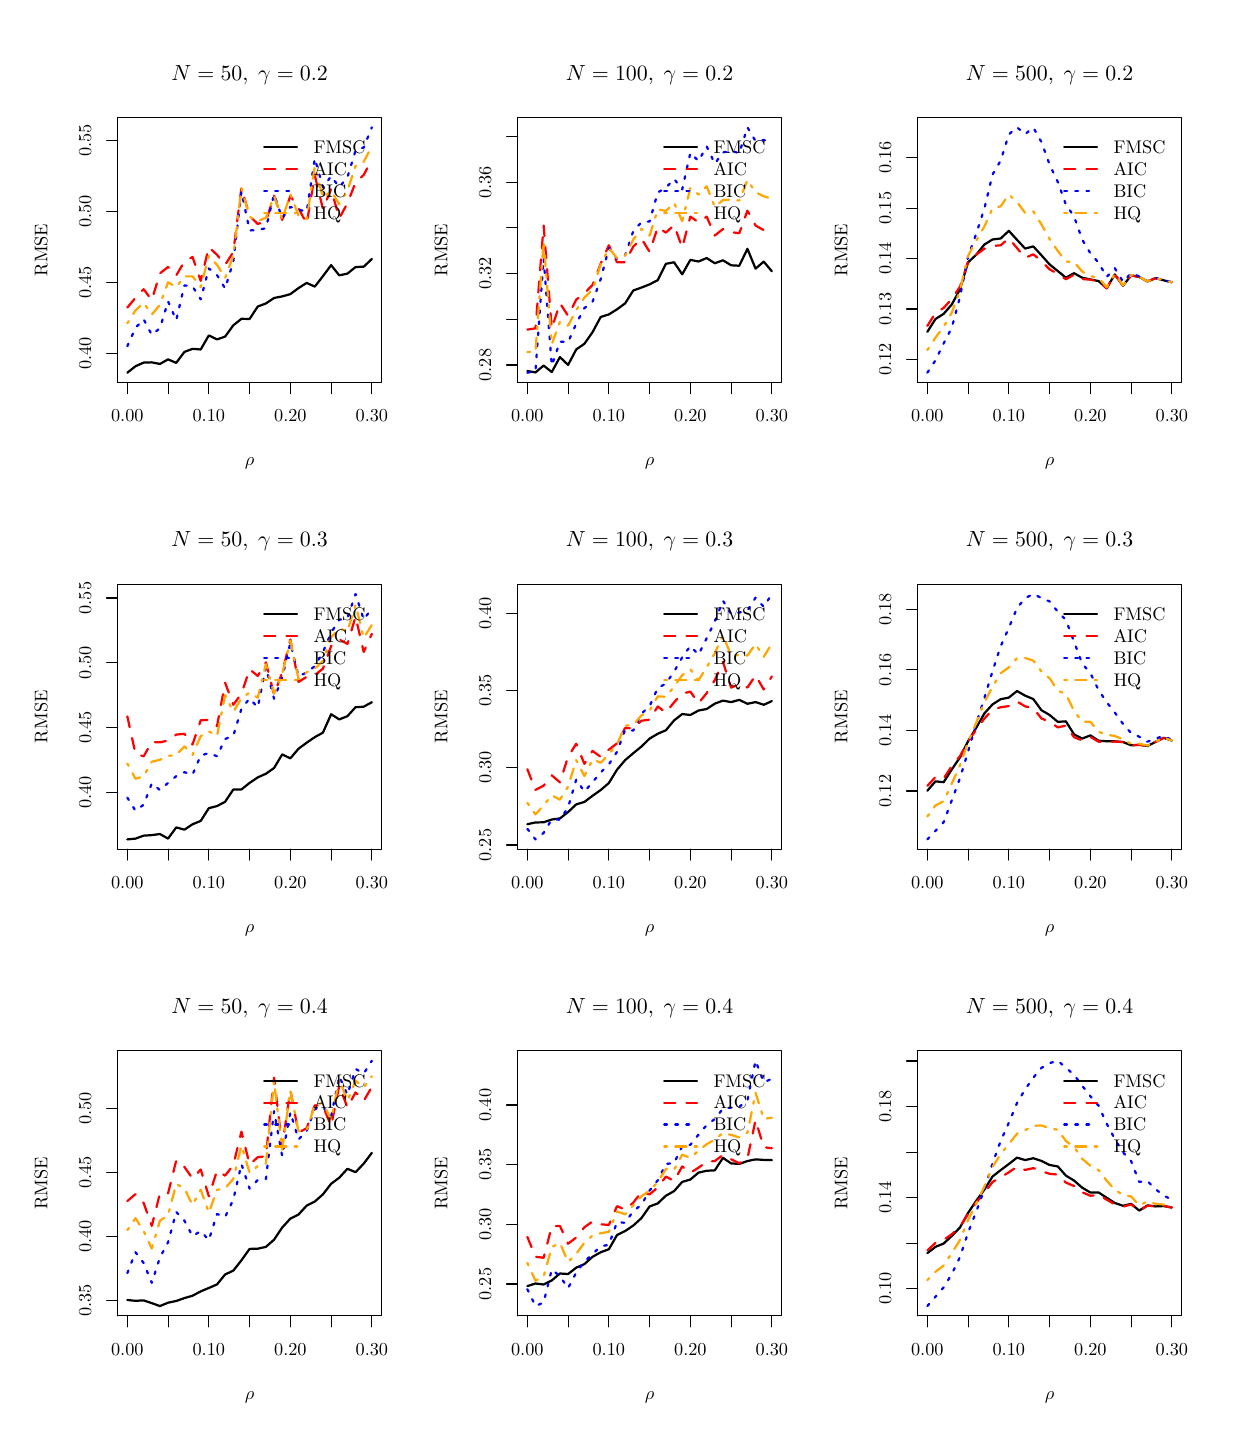
\begin{tikzpicture}[x=1pt,y=1pt]
\definecolor[named]{fillColor}{rgb}{1.00,1.00,1.00}
\path[use as bounding box,fill=fillColor,fill opacity=0.00] (0,0) rectangle (433.62,505.89);
\begin{scope}
\path[clip] ( 32.47,377.65) rectangle (127.91,473.42);
\definecolor[named]{drawColor}{rgb}{0.00,0.00,0.00}

\path[draw=drawColor,line width= 0.8pt,line join=round,line cap=round] ( 36.01,381.20) --
	( 38.95,383.53) --
	( 41.90,384.86) --
	( 44.84,384.95) --
	( 47.79,384.37) --
	( 50.73,386.03) --
	( 53.68,384.76) --
	( 56.63,388.72) --
	( 59.57,389.83) --
	( 62.52,389.60) --
	( 65.46,394.68) --
	( 68.41,393.25) --
	( 71.35,394.25) --
	( 74.30,398.34) --
	( 77.24,400.68) --
	( 80.19,400.63) --
	( 83.14,405.13) --
	( 86.08,406.23) --
	( 89.03,408.21) --
	( 91.97,408.78) --
	( 94.92,409.60) --
	( 97.86,411.78) --
	(100.81,413.65) --
	(103.75,412.32) --
	(106.70,416.10) --
	(109.65,420.08) --
	(112.59,416.38) --
	(115.54,417.02) --
	(118.48,419.39) --
	(121.43,419.52) --
	(124.37,422.30);
\end{scope}
\begin{scope}
\path[clip] (  0.00,  0.00) rectangle (433.62,505.89);
\definecolor[named]{drawColor}{rgb}{0.00,0.00,0.00}

\path[draw=drawColor,line width= 0.4pt,line join=round,line cap=round] ( 36.01,377.65) -- (124.37,377.65);

\path[draw=drawColor,line width= 0.4pt,line join=round,line cap=round] ( 36.01,377.65) -- ( 36.01,373.69);

\path[draw=drawColor,line width= 0.4pt,line join=round,line cap=round] ( 50.73,377.65) -- ( 50.73,373.69);

\path[draw=drawColor,line width= 0.4pt,line join=round,line cap=round] ( 65.46,377.65) -- ( 65.46,373.69);

\path[draw=drawColor,line width= 0.4pt,line join=round,line cap=round] ( 80.19,377.65) -- ( 80.19,373.69);

\path[draw=drawColor,line width= 0.4pt,line join=round,line cap=round] ( 94.92,377.65) -- ( 94.92,373.69);

\path[draw=drawColor,line width= 0.4pt,line join=round,line cap=round] (109.65,377.65) -- (109.65,373.69);

\path[draw=drawColor,line width= 0.4pt,line join=round,line cap=round] (124.37,377.65) -- (124.37,373.69);

\node[text=drawColor,anchor=base,inner sep=0pt, outer sep=0pt, scale=  0.66] at ( 36.01,363.40) {0.00};

\node[text=drawColor,anchor=base,inner sep=0pt, outer sep=0pt, scale=  0.66] at ( 65.46,363.40) {0.10};

\node[text=drawColor,anchor=base,inner sep=0pt, outer sep=0pt, scale=  0.66] at ( 94.92,363.40) {0.20};

\node[text=drawColor,anchor=base,inner sep=0pt, outer sep=0pt, scale=  0.66] at (124.37,363.40) {0.30};

\path[draw=drawColor,line width= 0.4pt,line join=round,line cap=round] ( 32.47,388.25) -- ( 32.47,465.04);

\path[draw=drawColor,line width= 0.4pt,line join=round,line cap=round] ( 32.47,388.25) -- ( 28.51,388.25);

\path[draw=drawColor,line width= 0.4pt,line join=round,line cap=round] ( 32.47,413.85) -- ( 28.51,413.85);

\path[draw=drawColor,line width= 0.4pt,line join=round,line cap=round] ( 32.47,439.44) -- ( 28.51,439.44);

\path[draw=drawColor,line width= 0.4pt,line join=round,line cap=round] ( 32.47,465.04) -- ( 28.51,465.04);

\node[text=drawColor,rotate= 90.00,anchor=base,inner sep=0pt, outer sep=0pt, scale=  0.66] at ( 22.97,388.25) {0.40};

\node[text=drawColor,rotate= 90.00,anchor=base,inner sep=0pt, outer sep=0pt, scale=  0.66] at ( 22.97,413.85) {0.45};

\node[text=drawColor,rotate= 90.00,anchor=base,inner sep=0pt, outer sep=0pt, scale=  0.66] at ( 22.97,439.44) {0.50};

\node[text=drawColor,rotate= 90.00,anchor=base,inner sep=0pt, outer sep=0pt, scale=  0.66] at ( 22.97,465.04) {0.55};

\path[draw=drawColor,line width= 0.4pt,line join=round,line cap=round] ( 32.47,377.65) --
	(127.91,377.65) --
	(127.91,473.42) --
	( 32.47,473.42) --
	( 32.47,377.65);
\end{scope}
\begin{scope}
\path[clip] (  0.00,337.26) rectangle (144.54,505.89);
\definecolor[named]{drawColor}{rgb}{0.00,0.00,0.00}

\node[text=drawColor,anchor=base,inner sep=0pt, outer sep=0pt, scale=  0.79] at ( 80.19,486.92) {\bfseries $N=50, \;\gamma=0.2$};

\node[text=drawColor,anchor=base,inner sep=0pt, outer sep=0pt, scale=  0.66] at ( 80.19,347.56) {$\rho$};

\node[text=drawColor,rotate= 90.00,anchor=base,inner sep=0pt, outer sep=0pt, scale=  0.66] at (  7.13,425.53) {RMSE};
\end{scope}
\begin{scope}
\path[clip] ( 32.47,377.65) rectangle (127.91,473.42);
\definecolor[named]{drawColor}{rgb}{1.00,0.00,0.00}

\path[draw=drawColor,line width= 0.8pt,dash pattern=on 4pt off 4pt ,line join=round,line cap=round] ( 36.01,404.76) --
	( 38.95,408.27) --
	( 41.90,411.37) --
	( 44.84,407.46) --
	( 47.79,417.10) --
	( 50.73,419.40) --
	( 53.68,416.37) --
	( 56.63,421.33) --
	( 59.57,423.04) --
	( 62.52,414.41) --
	( 65.46,426.57) --
	( 68.41,423.81) --
	( 71.35,420.17) --
	( 74.30,424.83) --
	( 77.24,448.09) --
	( 80.19,437.80) --
	( 83.14,434.95) --
	( 86.08,435.91) --
	( 89.03,445.25) --
	( 91.97,436.43) --
	( 94.92,445.06) --
	( 97.86,440.70) --
	(100.81,435.02) --
	(103.75,452.53) --
	(106.70,440.34) --
	(109.65,447.57) --
	(112.59,437.03) --
	(115.54,442.43) --
	(118.48,449.94) --
	(121.43,452.67) --
	(124.37,458.22);
\definecolor[named]{drawColor}{rgb}{0.00,0.00,1.00}

\path[draw=drawColor,line width= 0.8pt,dash pattern=on 1pt off 3pt ,line join=round,line cap=round] ( 36.01,390.78) --
	( 38.95,397.38) --
	( 41.90,400.54) --
	( 44.84,394.88) --
	( 47.79,397.29) --
	( 50.73,406.97) --
	( 53.68,400.18) --
	( 56.63,412.76) --
	( 59.57,412.39) --
	( 62.52,407.72) --
	( 65.46,418.86) --
	( 68.41,416.52) --
	( 71.35,411.63) --
	( 74.30,421.37) --
	( 77.24,446.64) --
	( 80.19,432.61) --
	( 83.14,432.76) --
	( 86.08,433.43) --
	( 89.03,445.70) --
	( 91.97,437.01) --
	( 94.92,441.12) --
	( 97.86,440.10) --
	(100.81,439.40) --
	(103.75,458.61) --
	(106.70,448.19) --
	(109.65,452.22) --
	(112.59,448.25) --
	(115.54,451.82) --
	(118.48,461.51) --
	(121.43,462.61) --
	(124.37,469.87);
\definecolor[named]{drawColor}{rgb}{1.00,0.65,0.00}

\path[draw=drawColor,line width= 0.8pt,dash pattern=on 1pt off 3pt on 4pt off 3pt ,line join=round,line cap=round] ( 36.01,399.03) --
	( 38.95,403.70) --
	( 41.90,406.51) --
	( 44.84,402.17) --
	( 47.79,405.76) --
	( 50.73,413.88) --
	( 53.68,412.10) --
	( 56.63,416.02) --
	( 59.57,416.02) --
	( 62.52,412.14) --
	( 65.46,423.43) --
	( 68.41,420.18) --
	( 71.35,415.45) --
	( 74.30,423.38) --
	( 77.24,447.86) --
	( 80.19,437.54) --
	( 83.14,436.05) --
	( 86.08,437.17) --
	( 89.03,445.04) --
	( 91.97,436.70) --
	( 94.92,445.65) --
	( 97.86,438.04) --
	(100.81,436.71) --
	(103.75,455.78) --
	(106.70,444.41) --
	(109.65,446.85) --
	(112.59,442.11) --
	(115.54,447.03) --
	(118.48,455.88) --
	(121.43,457.44) --
	(124.37,463.07);
\definecolor[named]{drawColor}{rgb}{0.00,0.00,0.00}

\path[draw=drawColor,line width= 0.8pt,line join=round,line cap=round] ( 85.47,462.63) -- ( 97.35,462.63);
\definecolor[named]{drawColor}{rgb}{1.00,0.00,0.00}

\path[draw=drawColor,line width= 0.8pt,dash pattern=on 4pt off 4pt ,line join=round,line cap=round] ( 85.47,454.71) -- ( 97.35,454.71);
\definecolor[named]{drawColor}{rgb}{0.00,0.00,1.00}

\path[draw=drawColor,line width= 0.8pt,dash pattern=on 1pt off 3pt ,line join=round,line cap=round] ( 85.47,446.79) -- ( 97.35,446.79);
\definecolor[named]{drawColor}{rgb}{1.00,0.65,0.00}

\path[draw=drawColor,line width= 0.8pt,dash pattern=on 1pt off 3pt on 4pt off 3pt ,line join=round,line cap=round] ( 85.47,438.87) -- ( 97.35,438.87);
\definecolor[named]{drawColor}{rgb}{0.00,0.00,0.00}

\node[text=drawColor,anchor=base west,inner sep=0pt, outer sep=0pt, scale=  0.66] at (103.29,460.35) {FMSC};

\node[text=drawColor,anchor=base west,inner sep=0pt, outer sep=0pt, scale=  0.66] at (103.29,452.43) {AIC};

\node[text=drawColor,anchor=base west,inner sep=0pt, outer sep=0pt, scale=  0.66] at (103.29,444.51) {BIC};

\node[text=drawColor,anchor=base west,inner sep=0pt, outer sep=0pt, scale=  0.66] at (103.29,436.59) {HQ};
\end{scope}
\begin{scope}
\path[clip] (177.01,377.65) rectangle (272.45,473.42);
\definecolor[named]{drawColor}{rgb}{0.00,0.00,0.00}

\path[draw=drawColor,line width= 0.8pt,line join=round,line cap=round] (180.55,381.82) --
	(183.49,381.31) --
	(186.44,383.78) --
	(189.38,381.44) --
	(192.33,386.86) --
	(195.27,384.01) --
	(198.22,389.61) --
	(201.17,391.66) --
	(204.11,395.85) --
	(207.06,401.34) --
	(210.00,402.27) --
	(212.95,404.11) --
	(215.89,406.26) --
	(218.84,410.92) --
	(221.78,411.97) --
	(224.73,413.13) --
	(227.68,414.66) --
	(230.62,420.55) --
	(233.57,421.11) --
	(236.51,416.76) --
	(239.46,421.97) --
	(242.40,421.39) --
	(245.35,422.64) --
	(248.29,420.76) --
	(251.24,421.83) --
	(254.19,420.02) --
	(257.13,419.86) --
	(260.08,425.97) --
	(263.02,418.81) --
	(265.97,421.34) --
	(268.91,417.85);
\end{scope}
\begin{scope}
\path[clip] (  0.00,  0.00) rectangle (433.62,505.89);
\definecolor[named]{drawColor}{rgb}{0.00,0.00,0.00}

\path[draw=drawColor,line width= 0.4pt,line join=round,line cap=round] (180.55,377.65) -- (268.91,377.65);

\path[draw=drawColor,line width= 0.4pt,line join=round,line cap=round] (180.55,377.65) -- (180.55,373.69);

\path[draw=drawColor,line width= 0.4pt,line join=round,line cap=round] (195.27,377.65) -- (195.27,373.69);

\path[draw=drawColor,line width= 0.4pt,line join=round,line cap=round] (210.00,377.65) -- (210.00,373.69);

\path[draw=drawColor,line width= 0.4pt,line join=round,line cap=round] (224.73,377.65) -- (224.73,373.69);

\path[draw=drawColor,line width= 0.4pt,line join=round,line cap=round] (239.46,377.65) -- (239.46,373.69);

\path[draw=drawColor,line width= 0.4pt,line join=round,line cap=round] (254.19,377.65) -- (254.19,373.69);

\path[draw=drawColor,line width= 0.4pt,line join=round,line cap=round] (268.91,377.65) -- (268.91,373.69);

\node[text=drawColor,anchor=base,inner sep=0pt, outer sep=0pt, scale=  0.66] at (180.55,363.40) {0.00};

\node[text=drawColor,anchor=base,inner sep=0pt, outer sep=0pt, scale=  0.66] at (210.00,363.40) {0.10};

\node[text=drawColor,anchor=base,inner sep=0pt, outer sep=0pt, scale=  0.66] at (239.46,363.40) {0.20};

\node[text=drawColor,anchor=base,inner sep=0pt, outer sep=0pt, scale=  0.66] at (268.91,363.40) {0.30};

\path[draw=drawColor,line width= 0.4pt,line join=round,line cap=round] (177.01,383.98) -- (177.01,466.56);

\path[draw=drawColor,line width= 0.4pt,line join=round,line cap=round] (177.01,383.98) -- (173.05,383.98);

\path[draw=drawColor,line width= 0.4pt,line join=round,line cap=round] (177.01,400.49) -- (173.05,400.49);

\path[draw=drawColor,line width= 0.4pt,line join=round,line cap=round] (177.01,417.01) -- (173.05,417.01);

\path[draw=drawColor,line width= 0.4pt,line join=round,line cap=round] (177.01,433.53) -- (173.05,433.53);

\path[draw=drawColor,line width= 0.4pt,line join=round,line cap=round] (177.01,450.04) -- (173.05,450.04);

\path[draw=drawColor,line width= 0.4pt,line join=round,line cap=round] (177.01,466.56) -- (173.05,466.56);

\node[text=drawColor,rotate= 90.00,anchor=base,inner sep=0pt, outer sep=0pt, scale=  0.66] at (167.51,383.98) {0.28};

\node[text=drawColor,rotate= 90.00,anchor=base,inner sep=0pt, outer sep=0pt, scale=  0.66] at (167.51,417.01) {0.32};

\node[text=drawColor,rotate= 90.00,anchor=base,inner sep=0pt, outer sep=0pt, scale=  0.66] at (167.51,450.04) {0.36};

\path[draw=drawColor,line width= 0.4pt,line join=round,line cap=round] (177.01,377.65) --
	(272.45,377.65) --
	(272.45,473.42) --
	(177.01,473.42) --
	(177.01,377.65);
\end{scope}
\begin{scope}
\path[clip] (144.54,337.26) rectangle (289.08,505.89);
\definecolor[named]{drawColor}{rgb}{0.00,0.00,0.00}

\node[text=drawColor,anchor=base,inner sep=0pt, outer sep=0pt, scale=  0.79] at (224.73,486.92) {\bfseries $N=100, \;\gamma=0.2$};

\node[text=drawColor,anchor=base,inner sep=0pt, outer sep=0pt, scale=  0.66] at (224.73,347.56) {$\rho$};

\node[text=drawColor,rotate= 90.00,anchor=base,inner sep=0pt, outer sep=0pt, scale=  0.66] at (151.67,425.53) {RMSE};
\end{scope}
\begin{scope}
\path[clip] (177.01,377.65) rectangle (272.45,473.42);
\definecolor[named]{drawColor}{rgb}{1.00,0.00,0.00}

\path[draw=drawColor,line width= 0.8pt,dash pattern=on 4pt off 4pt ,line join=round,line cap=round] (180.55,396.78) --
	(183.49,397.24) --
	(186.44,434.38) --
	(189.38,397.22) --
	(192.33,406.30) --
	(195.27,401.77) --
	(198.22,407.60) --
	(201.17,409.93) --
	(204.11,412.91) --
	(207.06,420.60) --
	(210.00,427.25) --
	(212.95,421.10) --
	(215.89,421.16) --
	(218.84,426.80) --
	(221.78,429.68) --
	(224.73,424.88) --
	(227.68,433.79) --
	(230.62,431.82) --
	(233.57,434.58) --
	(236.51,426.42) --
	(239.46,437.61) --
	(242.40,435.56) --
	(245.35,437.59) --
	(248.29,430.79) --
	(251.24,433.12) --
	(254.19,432.01) --
	(257.13,431.61) --
	(260.08,439.75) --
	(263.02,434.38) --
	(265.97,432.72) --
	(268.91,431.68);
\definecolor[named]{drawColor}{rgb}{0.00,0.00,1.00}

\path[draw=drawColor,line width= 0.8pt,dash pattern=on 1pt off 3pt ,line join=round,line cap=round] (180.55,381.20) --
	(183.49,381.79) --
	(186.44,422.43) --
	(189.38,383.78) --
	(192.33,392.44) --
	(195.27,392.27) --
	(198.22,398.91) --
	(201.17,404.57) --
	(204.11,406.83) --
	(207.06,415.04) --
	(210.00,426.17) --
	(212.95,422.44) --
	(215.89,423.65) --
	(218.84,432.39) --
	(221.78,435.57) --
	(224.73,435.87) --
	(227.68,446.36) --
	(230.62,447.99) --
	(233.57,451.25) --
	(236.51,447.44) --
	(239.46,460.68) --
	(242.40,457.69) --
	(245.35,462.98) --
	(248.29,456.74) --
	(251.24,460.78) --
	(254.19,461.40) --
	(257.13,460.49) --
	(260.08,469.87) --
	(263.02,464.90) --
	(265.97,465.31) --
	(268.91,464.31);
\definecolor[named]{drawColor}{rgb}{1.00,0.65,0.00}

\path[draw=drawColor,line width= 0.8pt,dash pattern=on 1pt off 3pt on 4pt off 3pt ,line join=round,line cap=round] (180.55,388.68) --
	(183.49,388.85) --
	(186.44,428.73) --
	(189.38,391.43) --
	(192.33,399.62) --
	(195.27,398.20) --
	(198.22,403.83) --
	(201.17,408.38) --
	(204.11,411.18) --
	(207.06,420.31) --
	(210.00,426.23) --
	(212.95,422.67) --
	(215.89,423.51) --
	(218.84,429.35) --
	(221.78,433.18) --
	(224.73,430.73) --
	(227.68,440.28) --
	(230.62,439.63) --
	(233.57,442.58) --
	(236.51,435.97) --
	(239.46,447.95) --
	(242.40,445.61) --
	(245.35,448.57) --
	(248.29,441.10) --
	(251.24,443.60) --
	(254.19,443.72) --
	(257.13,443.42) --
	(260.08,450.84) --
	(263.02,446.41) --
	(265.97,444.95) --
	(268.91,444.09);
\definecolor[named]{drawColor}{rgb}{0.00,0.00,0.00}

\path[draw=drawColor,line width= 0.8pt,line join=round,line cap=round] (230.01,462.63) -- (241.89,462.63);
\definecolor[named]{drawColor}{rgb}{1.00,0.00,0.00}

\path[draw=drawColor,line width= 0.8pt,dash pattern=on 4pt off 4pt ,line join=round,line cap=round] (230.01,454.71) -- (241.89,454.71);
\definecolor[named]{drawColor}{rgb}{0.00,0.00,1.00}

\path[draw=drawColor,line width= 0.8pt,dash pattern=on 1pt off 3pt ,line join=round,line cap=round] (230.01,446.79) -- (241.89,446.79);
\definecolor[named]{drawColor}{rgb}{1.00,0.65,0.00}

\path[draw=drawColor,line width= 0.8pt,dash pattern=on 1pt off 3pt on 4pt off 3pt ,line join=round,line cap=round] (230.01,438.87) -- (241.89,438.87);
\definecolor[named]{drawColor}{rgb}{0.00,0.00,0.00}

\node[text=drawColor,anchor=base west,inner sep=0pt, outer sep=0pt, scale=  0.66] at (247.83,460.35) {FMSC};

\node[text=drawColor,anchor=base west,inner sep=0pt, outer sep=0pt, scale=  0.66] at (247.83,452.43) {AIC};

\node[text=drawColor,anchor=base west,inner sep=0pt, outer sep=0pt, scale=  0.66] at (247.83,444.51) {BIC};

\node[text=drawColor,anchor=base west,inner sep=0pt, outer sep=0pt, scale=  0.66] at (247.83,436.59) {HQ};
\end{scope}
\begin{scope}
\path[clip] (321.55,377.65) rectangle (416.99,473.42);
\definecolor[named]{drawColor}{rgb}{0.00,0.00,0.00}

\path[draw=drawColor,line width= 0.8pt,line join=round,line cap=round] (325.09,395.97) --
	(328.03,400.60) --
	(330.98,402.47) --
	(333.92,405.85) --
	(336.87,411.31) --
	(339.81,421.09) --
	(342.76,423.85) --
	(345.71,427.53) --
	(348.65,429.35) --
	(351.60,429.71) --
	(354.54,432.47) --
	(357.49,429.23) --
	(360.43,426.06) --
	(363.38,426.85) --
	(366.32,423.64) --
	(369.27,420.33) --
	(372.22,417.96) --
	(375.16,415.54) --
	(378.11,417.16) --
	(381.05,415.53) --
	(384.00,414.91) --
	(386.94,414.32) --
	(389.89,411.75) --
	(392.83,416.73) --
	(395.78,412.64) --
	(398.73,416.37) --
	(401.67,415.78) --
	(404.62,414.18) --
	(407.56,415.37) --
	(410.51,414.58) --
	(413.45,413.90);
\end{scope}
\begin{scope}
\path[clip] (  0.00,  0.00) rectangle (433.62,505.89);
\definecolor[named]{drawColor}{rgb}{0.00,0.00,0.00}

\path[draw=drawColor,line width= 0.4pt,line join=round,line cap=round] (325.09,377.65) -- (413.45,377.65);

\path[draw=drawColor,line width= 0.4pt,line join=round,line cap=round] (325.09,377.65) -- (325.09,373.69);

\path[draw=drawColor,line width= 0.4pt,line join=round,line cap=round] (339.81,377.65) -- (339.81,373.69);

\path[draw=drawColor,line width= 0.4pt,line join=round,line cap=round] (354.54,377.65) -- (354.54,373.69);

\path[draw=drawColor,line width= 0.4pt,line join=round,line cap=round] (369.27,377.65) -- (369.27,373.69);

\path[draw=drawColor,line width= 0.4pt,line join=round,line cap=round] (384.00,377.65) -- (384.00,373.69);

\path[draw=drawColor,line width= 0.4pt,line join=round,line cap=round] (398.73,377.65) -- (398.73,373.69);

\path[draw=drawColor,line width= 0.4pt,line join=round,line cap=round] (413.45,377.65) -- (413.45,373.69);

\node[text=drawColor,anchor=base,inner sep=0pt, outer sep=0pt, scale=  0.66] at (325.09,363.40) {0.00};

\node[text=drawColor,anchor=base,inner sep=0pt, outer sep=0pt, scale=  0.66] at (354.54,363.40) {0.10};

\node[text=drawColor,anchor=base,inner sep=0pt, outer sep=0pt, scale=  0.66] at (384.00,363.40) {0.20};

\node[text=drawColor,anchor=base,inner sep=0pt, outer sep=0pt, scale=  0.66] at (413.45,363.40) {0.30};

\path[draw=drawColor,line width= 0.4pt,line join=round,line cap=round] (321.55,385.99) -- (321.55,458.94);

\path[draw=drawColor,line width= 0.4pt,line join=round,line cap=round] (321.55,385.99) -- (317.59,385.99);

\path[draw=drawColor,line width= 0.4pt,line join=round,line cap=round] (321.55,404.23) -- (317.59,404.23);

\path[draw=drawColor,line width= 0.4pt,line join=round,line cap=round] (321.55,422.47) -- (317.59,422.47);

\path[draw=drawColor,line width= 0.4pt,line join=round,line cap=round] (321.55,440.70) -- (317.59,440.70);

\path[draw=drawColor,line width= 0.4pt,line join=round,line cap=round] (321.55,458.94) -- (317.59,458.94);

\node[text=drawColor,rotate= 90.00,anchor=base,inner sep=0pt, outer sep=0pt, scale=  0.66] at (312.05,385.99) {0.12};

\node[text=drawColor,rotate= 90.00,anchor=base,inner sep=0pt, outer sep=0pt, scale=  0.66] at (312.05,404.23) {0.13};

\node[text=drawColor,rotate= 90.00,anchor=base,inner sep=0pt, outer sep=0pt, scale=  0.66] at (312.05,422.47) {0.14};

\node[text=drawColor,rotate= 90.00,anchor=base,inner sep=0pt, outer sep=0pt, scale=  0.66] at (312.05,440.70) {0.15};

\node[text=drawColor,rotate= 90.00,anchor=base,inner sep=0pt, outer sep=0pt, scale=  0.66] at (312.05,458.94) {0.16};

\path[draw=drawColor,line width= 0.4pt,line join=round,line cap=round] (321.55,377.65) --
	(416.99,377.65) --
	(416.99,473.42) --
	(321.55,473.42) --
	(321.55,377.65);
\end{scope}
\begin{scope}
\path[clip] (289.08,337.26) rectangle (433.62,505.89);
\definecolor[named]{drawColor}{rgb}{0.00,0.00,0.00}

\node[text=drawColor,anchor=base,inner sep=0pt, outer sep=0pt, scale=  0.79] at (369.27,486.92) {\bfseries $N=500, \;\gamma=0.2$};

\node[text=drawColor,anchor=base,inner sep=0pt, outer sep=0pt, scale=  0.66] at (369.27,347.56) {$\rho$};

\node[text=drawColor,rotate= 90.00,anchor=base,inner sep=0pt, outer sep=0pt, scale=  0.66] at (296.21,425.53) {RMSE};
\end{scope}
\begin{scope}
\path[clip] (321.55,377.65) rectangle (416.99,473.42);
\definecolor[named]{drawColor}{rgb}{1.00,0.00,0.00}

\path[draw=drawColor,line width= 0.8pt,dash pattern=on 4pt off 4pt ,line join=round,line cap=round] (325.09,398.10) --
	(328.03,402.78) --
	(330.98,404.62) --
	(333.92,407.86) --
	(336.87,412.23) --
	(339.81,421.41) --
	(342.76,423.86) --
	(345.71,426.02) --
	(348.65,427.00) --
	(351.60,427.25) --
	(354.54,429.78) --
	(357.49,426.25) --
	(360.43,422.71) --
	(363.38,423.99) --
	(366.32,421.56) --
	(369.27,418.55) --
	(372.22,416.96) --
	(375.16,414.97) --
	(378.11,416.64) --
	(381.05,415.05) --
	(384.00,414.82) --
	(386.94,414.19) --
	(389.89,411.71) --
	(392.83,416.73) --
	(395.78,412.64) --
	(398.73,416.37) --
	(401.67,415.78) --
	(404.62,414.18) --
	(407.56,415.37) --
	(410.51,414.58) --
	(413.45,413.90);
\definecolor[named]{drawColor}{rgb}{0.00,0.00,1.00}

\path[draw=drawColor,line width= 0.8pt,dash pattern=on 1pt off 3pt ,line join=round,line cap=round] (325.09,381.20) --
	(328.03,385.69) --
	(330.98,391.78) --
	(333.92,397.46) --
	(336.87,408.52) --
	(339.81,423.17) --
	(342.76,431.44) --
	(345.71,440.59) --
	(348.65,452.81) --
	(351.60,457.87) --
	(354.54,467.33) --
	(357.49,469.87) --
	(360.43,467.42) --
	(363.38,469.80) --
	(366.32,464.56) --
	(369.27,456.40) --
	(372.22,450.17) --
	(375.16,441.93) --
	(378.11,437.66) --
	(381.05,429.30) --
	(384.00,424.36) --
	(386.94,421.00) --
	(389.89,415.82) --
	(392.83,418.95) --
	(395.78,414.08) --
	(398.73,417.17) --
	(401.67,415.99) --
	(404.62,414.25) --
	(407.56,415.44) --
	(410.51,414.60) --
	(413.45,413.90);
\definecolor[named]{drawColor}{rgb}{1.00,0.65,0.00}

\path[draw=drawColor,line width= 0.8pt,dash pattern=on 1pt off 3pt on 4pt off 3pt ,line join=round,line cap=round] (325.09,389.38) --
	(328.03,393.91) --
	(330.98,397.78) --
	(333.92,402.95) --
	(336.87,410.89) --
	(339.81,423.45) --
	(342.76,428.99) --
	(345.71,434.05) --
	(348.65,440.60) --
	(351.60,441.34) --
	(354.54,445.62) --
	(357.49,442.90) --
	(360.43,438.95) --
	(363.38,439.49) --
	(366.32,434.80) --
	(369.27,429.48) --
	(372.22,425.21) --
	(375.16,421.38) --
	(378.11,421.20) --
	(381.05,417.76) --
	(384.00,416.14) --
	(386.94,415.46) --
	(389.89,412.12) --
	(392.83,416.92) --
	(395.78,412.76) --
	(398.73,416.52) --
	(401.67,415.85) --
	(404.62,414.18) --
	(407.56,415.37) --
	(410.51,414.58) --
	(413.45,413.90);
\definecolor[named]{drawColor}{rgb}{0.00,0.00,0.00}

\path[draw=drawColor,line width= 0.8pt,line join=round,line cap=round] (374.55,462.63) -- (386.43,462.63);
\definecolor[named]{drawColor}{rgb}{1.00,0.00,0.00}

\path[draw=drawColor,line width= 0.8pt,dash pattern=on 4pt off 4pt ,line join=round,line cap=round] (374.55,454.71) -- (386.43,454.71);
\definecolor[named]{drawColor}{rgb}{0.00,0.00,1.00}

\path[draw=drawColor,line width= 0.8pt,dash pattern=on 1pt off 3pt ,line join=round,line cap=round] (374.55,446.79) -- (386.43,446.79);
\definecolor[named]{drawColor}{rgb}{1.00,0.65,0.00}

\path[draw=drawColor,line width= 0.8pt,dash pattern=on 1pt off 3pt on 4pt off 3pt ,line join=round,line cap=round] (374.55,438.87) -- (386.43,438.87);
\definecolor[named]{drawColor}{rgb}{0.00,0.00,0.00}

\node[text=drawColor,anchor=base west,inner sep=0pt, outer sep=0pt, scale=  0.66] at (392.37,460.35) {FMSC};

\node[text=drawColor,anchor=base west,inner sep=0pt, outer sep=0pt, scale=  0.66] at (392.37,452.43) {AIC};

\node[text=drawColor,anchor=base west,inner sep=0pt, outer sep=0pt, scale=  0.66] at (392.37,444.51) {BIC};

\node[text=drawColor,anchor=base west,inner sep=0pt, outer sep=0pt, scale=  0.66] at (392.37,436.59) {HQ};
\end{scope}
\begin{scope}
\path[clip] ( 32.47,209.02) rectangle (127.91,304.79);
\definecolor[named]{drawColor}{rgb}{0.00,0.00,0.00}

\path[draw=drawColor,line width= 0.8pt,line join=round,line cap=round] ( 36.01,212.57) --
	( 38.95,212.85) --
	( 41.90,213.92) --
	( 44.84,214.12) --
	( 47.79,214.51) --
	( 50.73,212.86) --
	( 53.68,216.91) --
	( 56.63,216.09) --
	( 59.57,218.04) --
	( 62.52,219.24) --
	( 65.46,223.85) --
	( 68.41,224.61) --
	( 71.35,226.16) --
	( 74.30,230.59) --
	( 77.24,230.62) --
	( 80.19,232.97) --
	( 83.14,234.98) --
	( 86.08,236.29) --
	( 89.03,238.36) --
	( 91.97,243.28) --
	( 94.92,241.85) --
	( 97.86,245.34) --
	(100.81,247.50) --
	(103.75,249.52) --
	(106.70,251.16) --
	(109.65,257.79) --
	(112.59,255.93) --
	(115.54,257.09) --
	(118.48,260.34) --
	(121.43,260.52) --
	(124.37,262.14);
\end{scope}
\begin{scope}
\path[clip] (  0.00,  0.00) rectangle (433.62,505.89);
\definecolor[named]{drawColor}{rgb}{0.00,0.00,0.00}

\path[draw=drawColor,line width= 0.4pt,line join=round,line cap=round] ( 36.01,209.02) -- (124.37,209.02);

\path[draw=drawColor,line width= 0.4pt,line join=round,line cap=round] ( 36.01,209.02) -- ( 36.01,205.06);

\path[draw=drawColor,line width= 0.4pt,line join=round,line cap=round] ( 50.73,209.02) -- ( 50.73,205.06);

\path[draw=drawColor,line width= 0.4pt,line join=round,line cap=round] ( 65.46,209.02) -- ( 65.46,205.06);

\path[draw=drawColor,line width= 0.4pt,line join=round,line cap=round] ( 80.19,209.02) -- ( 80.19,205.06);

\path[draw=drawColor,line width= 0.4pt,line join=round,line cap=round] ( 94.92,209.02) -- ( 94.92,205.06);

\path[draw=drawColor,line width= 0.4pt,line join=round,line cap=round] (109.65,209.02) -- (109.65,205.06);

\path[draw=drawColor,line width= 0.4pt,line join=round,line cap=round] (124.37,209.02) -- (124.37,205.06);

\node[text=drawColor,anchor=base,inner sep=0pt, outer sep=0pt, scale=  0.66] at ( 36.01,194.77) {0.00};

\node[text=drawColor,anchor=base,inner sep=0pt, outer sep=0pt, scale=  0.66] at ( 65.46,194.77) {0.10};

\node[text=drawColor,anchor=base,inner sep=0pt, outer sep=0pt, scale=  0.66] at ( 94.92,194.77) {0.20};

\node[text=drawColor,anchor=base,inner sep=0pt, outer sep=0pt, scale=  0.66] at (124.37,194.77) {0.30};

\path[draw=drawColor,line width= 0.4pt,line join=round,line cap=round] ( 32.47,229.61) -- ( 32.47,299.78);

\path[draw=drawColor,line width= 0.4pt,line join=round,line cap=round] ( 32.47,229.61) -- ( 28.51,229.61);

\path[draw=drawColor,line width= 0.4pt,line join=round,line cap=round] ( 32.47,253.00) -- ( 28.51,253.00);

\path[draw=drawColor,line width= 0.4pt,line join=round,line cap=round] ( 32.47,276.39) -- ( 28.51,276.39);

\path[draw=drawColor,line width= 0.4pt,line join=round,line cap=round] ( 32.47,299.78) -- ( 28.51,299.78);

\node[text=drawColor,rotate= 90.00,anchor=base,inner sep=0pt, outer sep=0pt, scale=  0.66] at ( 22.97,229.61) {0.40};

\node[text=drawColor,rotate= 90.00,anchor=base,inner sep=0pt, outer sep=0pt, scale=  0.66] at ( 22.97,253.00) {0.45};

\node[text=drawColor,rotate= 90.00,anchor=base,inner sep=0pt, outer sep=0pt, scale=  0.66] at ( 22.97,276.39) {0.50};

\node[text=drawColor,rotate= 90.00,anchor=base,inner sep=0pt, outer sep=0pt, scale=  0.66] at ( 22.97,299.78) {0.55};

\path[draw=drawColor,line width= 0.4pt,line join=round,line cap=round] ( 32.47,209.02) --
	(127.91,209.02) --
	(127.91,304.79) --
	( 32.47,304.79) --
	( 32.47,209.02);
\end{scope}
\begin{scope}
\path[clip] (  0.00,168.63) rectangle (144.54,337.26);
\definecolor[named]{drawColor}{rgb}{0.00,0.00,0.00}

\node[text=drawColor,anchor=base,inner sep=0pt, outer sep=0pt, scale=  0.79] at ( 80.19,318.29) {\bfseries $N=50, \;\gamma=0.3$};

\node[text=drawColor,anchor=base,inner sep=0pt, outer sep=0pt, scale=  0.66] at ( 80.19,178.93) {$\rho$};

\node[text=drawColor,rotate= 90.00,anchor=base,inner sep=0pt, outer sep=0pt, scale=  0.66] at (  7.13,256.90) {RMSE};
\end{scope}
\begin{scope}
\path[clip] ( 32.47,209.02) rectangle (127.91,304.79);
\definecolor[named]{drawColor}{rgb}{1.00,0.00,0.00}

\path[draw=drawColor,line width= 0.8pt,dash pattern=on 4pt off 4pt ,line join=round,line cap=round] ( 36.01,257.02) --
	( 38.95,243.55) --
	( 41.90,242.58) --
	( 44.84,247.78) --
	( 47.79,247.63) --
	( 50.73,248.30) --
	( 53.68,250.43) --
	( 56.63,250.72) --
	( 59.57,246.84) --
	( 62.52,255.61) --
	( 65.46,255.78) --
	( 68.41,253.48) --
	( 71.35,269.17) --
	( 74.30,261.21) --
	( 77.24,265.23) --
	( 80.19,274.03) --
	( 83.14,271.63) --
	( 86.08,276.53) --
	( 89.03,264.92) --
	( 91.97,272.84) --
	( 94.92,284.81) --
	( 97.86,269.47) --
	(100.81,271.32) --
	(103.75,271.95) --
	(106.70,274.28) --
	(109.65,282.42) --
	(112.59,284.83) --
	(115.54,283.20) --
	(118.48,293.02) --
	(121.43,280.30) --
	(124.37,286.87);
\definecolor[named]{drawColor}{rgb}{0.00,0.00,1.00}

\path[draw=drawColor,line width= 0.8pt,dash pattern=on 1pt off 3pt ,line join=round,line cap=round] ( 36.01,227.65) --
	( 38.95,222.93) --
	( 41.90,225.10) --
	( 44.84,232.77) --
	( 47.79,230.40) --
	( 50.73,233.00) --
	( 53.68,235.41) --
	( 56.63,236.84) --
	( 59.57,235.99) --
	( 62.52,242.86) --
	( 65.46,243.79) --
	( 68.41,242.62) --
	( 71.35,248.85) --
	( 74.30,250.00) --
	( 77.24,259.75) --
	( 80.19,263.50) --
	( 83.14,260.27) --
	( 86.08,274.73) --
	( 89.03,263.39) --
	( 91.97,271.00) --
	( 94.92,283.59) --
	( 97.86,271.54) --
	(100.81,272.86) --
	(103.75,275.17) --
	(106.70,280.27) --
	(109.65,287.25) --
	(112.59,291.94) --
	(115.54,292.52) --
	(118.48,301.24) --
	(121.43,291.98) --
	(124.37,296.12);
\definecolor[named]{drawColor}{rgb}{1.00,0.65,0.00}

\path[draw=drawColor,line width= 0.8pt,dash pattern=on 1pt off 3pt on 4pt off 3pt ,line join=round,line cap=round] ( 36.01,240.01) --
	( 38.95,234.49) --
	( 41.90,235.34) --
	( 44.84,240.63) --
	( 47.79,241.34) --
	( 50.73,242.72) --
	( 53.68,243.09) --
	( 56.63,246.17) --
	( 59.57,243.13) --
	( 62.52,249.85) --
	( 65.46,251.59) --
	( 68.41,249.96) --
	( 71.35,264.77) --
	( 74.30,258.65) --
	( 77.24,263.56) --
	( 80.19,265.64) --
	( 83.14,263.75) --
	( 86.08,275.89) --
	( 89.03,265.22) --
	( 91.97,272.44) --
	( 94.92,284.37) --
	( 97.86,270.55) --
	(100.81,272.92) --
	(103.75,274.30) --
	(106.70,277.12) --
	(109.65,285.58) --
	(112.59,288.74) --
	(115.54,287.79) --
	(118.48,297.33) --
	(121.43,285.36) --
	(124.37,290.11);
\definecolor[named]{drawColor}{rgb}{0.00,0.00,0.00}

\path[draw=drawColor,line width= 0.8pt,line join=round,line cap=round] ( 85.47,294.00) -- ( 97.35,294.00);
\definecolor[named]{drawColor}{rgb}{1.00,0.00,0.00}

\path[draw=drawColor,line width= 0.8pt,dash pattern=on 4pt off 4pt ,line join=round,line cap=round] ( 85.47,286.08) -- ( 97.35,286.08);
\definecolor[named]{drawColor}{rgb}{0.00,0.00,1.00}

\path[draw=drawColor,line width= 0.8pt,dash pattern=on 1pt off 3pt ,line join=round,line cap=round] ( 85.47,278.16) -- ( 97.35,278.16);
\definecolor[named]{drawColor}{rgb}{1.00,0.65,0.00}

\path[draw=drawColor,line width= 0.8pt,dash pattern=on 1pt off 3pt on 4pt off 3pt ,line join=round,line cap=round] ( 85.47,270.24) -- ( 97.35,270.24);
\definecolor[named]{drawColor}{rgb}{0.00,0.00,0.00}

\node[text=drawColor,anchor=base west,inner sep=0pt, outer sep=0pt, scale=  0.66] at (103.29,291.72) {FMSC};

\node[text=drawColor,anchor=base west,inner sep=0pt, outer sep=0pt, scale=  0.66] at (103.29,283.80) {AIC};

\node[text=drawColor,anchor=base west,inner sep=0pt, outer sep=0pt, scale=  0.66] at (103.29,275.88) {BIC};

\node[text=drawColor,anchor=base west,inner sep=0pt, outer sep=0pt, scale=  0.66] at (103.29,267.96) {HQ};
\end{scope}
\begin{scope}
\path[clip] (177.01,209.02) rectangle (272.45,304.79);
\definecolor[named]{drawColor}{rgb}{0.00,0.00,0.00}

\path[draw=drawColor,line width= 0.8pt,line join=round,line cap=round] (180.55,218.06) --
	(183.49,218.69) --
	(186.44,218.75) --
	(189.38,219.76) --
	(192.33,220.15) --
	(195.27,222.44) --
	(198.22,225.23) --
	(201.17,226.10) --
	(204.11,228.33) --
	(207.06,230.41) --
	(210.00,232.94) --
	(212.95,237.74) --
	(215.89,241.21) --
	(218.84,243.72) --
	(221.78,246.12) --
	(224.73,248.99) --
	(227.68,250.74) --
	(230.62,252.01) --
	(233.57,255.56) --
	(236.51,257.86) --
	(239.46,257.53) --
	(242.40,259.13) --
	(245.35,259.70) --
	(248.29,261.62) --
	(251.24,262.72) --
	(254.19,262.17) --
	(257.13,263.00) --
	(260.08,261.57) --
	(263.02,262.19) --
	(265.97,261.20) --
	(268.91,262.55);
\end{scope}
\begin{scope}
\path[clip] (  0.00,  0.00) rectangle (433.62,505.89);
\definecolor[named]{drawColor}{rgb}{0.00,0.00,0.00}

\path[draw=drawColor,line width= 0.4pt,line join=round,line cap=round] (180.55,209.02) -- (268.91,209.02);

\path[draw=drawColor,line width= 0.4pt,line join=round,line cap=round] (180.55,209.02) -- (180.55,205.06);

\path[draw=drawColor,line width= 0.4pt,line join=round,line cap=round] (195.27,209.02) -- (195.27,205.06);

\path[draw=drawColor,line width= 0.4pt,line join=round,line cap=round] (210.00,209.02) -- (210.00,205.06);

\path[draw=drawColor,line width= 0.4pt,line join=round,line cap=round] (224.73,209.02) -- (224.73,205.06);

\path[draw=drawColor,line width= 0.4pt,line join=round,line cap=round] (239.46,209.02) -- (239.46,205.06);

\path[draw=drawColor,line width= 0.4pt,line join=round,line cap=round] (254.19,209.02) -- (254.19,205.06);

\path[draw=drawColor,line width= 0.4pt,line join=round,line cap=round] (268.91,209.02) -- (268.91,205.06);

\node[text=drawColor,anchor=base,inner sep=0pt, outer sep=0pt, scale=  0.66] at (180.55,194.77) {0.00};

\node[text=drawColor,anchor=base,inner sep=0pt, outer sep=0pt, scale=  0.66] at (210.00,194.77) {0.10};

\node[text=drawColor,anchor=base,inner sep=0pt, outer sep=0pt, scale=  0.66] at (239.46,194.77) {0.20};

\node[text=drawColor,anchor=base,inner sep=0pt, outer sep=0pt, scale=  0.66] at (268.91,194.77) {0.30};

\path[draw=drawColor,line width= 0.4pt,line join=round,line cap=round] (177.01,210.54) -- (177.01,294.31);

\path[draw=drawColor,line width= 0.4pt,line join=round,line cap=round] (177.01,210.54) -- (173.05,210.54);

\path[draw=drawColor,line width= 0.4pt,line join=round,line cap=round] (177.01,238.47) -- (173.05,238.47);

\path[draw=drawColor,line width= 0.4pt,line join=round,line cap=round] (177.01,266.39) -- (173.05,266.39);

\path[draw=drawColor,line width= 0.4pt,line join=round,line cap=round] (177.01,294.31) -- (173.05,294.31);

\node[text=drawColor,rotate= 90.00,anchor=base,inner sep=0pt, outer sep=0pt, scale=  0.66] at (167.51,210.54) {0.25};

\node[text=drawColor,rotate= 90.00,anchor=base,inner sep=0pt, outer sep=0pt, scale=  0.66] at (167.51,238.47) {0.30};

\node[text=drawColor,rotate= 90.00,anchor=base,inner sep=0pt, outer sep=0pt, scale=  0.66] at (167.51,266.39) {0.35};

\node[text=drawColor,rotate= 90.00,anchor=base,inner sep=0pt, outer sep=0pt, scale=  0.66] at (167.51,294.31) {0.40};

\path[draw=drawColor,line width= 0.4pt,line join=round,line cap=round] (177.01,209.02) --
	(272.45,209.02) --
	(272.45,304.79) --
	(177.01,304.79) --
	(177.01,209.02);
\end{scope}
\begin{scope}
\path[clip] (144.54,168.63) rectangle (289.08,337.26);
\definecolor[named]{drawColor}{rgb}{0.00,0.00,0.00}

\node[text=drawColor,anchor=base,inner sep=0pt, outer sep=0pt, scale=  0.79] at (224.73,318.29) {\bfseries $N=100, \;\gamma=0.3$};

\node[text=drawColor,anchor=base,inner sep=0pt, outer sep=0pt, scale=  0.66] at (224.73,178.93) {$\rho$};

\node[text=drawColor,rotate= 90.00,anchor=base,inner sep=0pt, outer sep=0pt, scale=  0.66] at (151.67,256.90) {RMSE};
\end{scope}
\begin{scope}
\path[clip] (177.01,209.02) rectangle (272.45,304.79);
\definecolor[named]{drawColor}{rgb}{1.00,0.00,0.00}

\path[draw=drawColor,line width= 0.8pt,dash pattern=on 4pt off 4pt ,line join=round,line cap=round] (180.55,237.94) --
	(183.49,230.46) --
	(186.44,232.00) --
	(189.38,235.71) --
	(192.33,233.18) --
	(195.27,242.43) --
	(198.22,247.15) --
	(201.17,239.86) --
	(204.11,244.55) --
	(207.06,242.38) --
	(210.00,245.01) --
	(212.95,247.26) --
	(215.89,252.83) --
	(218.84,252.71) --
	(221.78,255.44) --
	(224.73,255.84) --
	(227.68,260.60) --
	(230.62,258.33) --
	(233.57,262.11) --
	(236.51,265.29) --
	(239.46,265.95) --
	(242.40,261.78) --
	(245.35,265.42) --
	(248.29,270.14) --
	(251.24,276.73) --
	(254.19,267.41) --
	(257.13,268.66) --
	(260.08,267.46) --
	(263.02,271.86) --
	(265.97,266.76) --
	(268.91,271.46);
\definecolor[named]{drawColor}{rgb}{0.00,0.00,1.00}

\path[draw=drawColor,line width= 0.8pt,dash pattern=on 1pt off 3pt ,line join=round,line cap=round] (180.55,216.41) --
	(183.49,212.57) --
	(186.44,214.94) --
	(189.38,219.79) --
	(192.33,219.69) --
	(195.27,224.10) --
	(198.22,234.23) --
	(201.17,229.82) --
	(204.11,233.25) --
	(207.06,236.76) --
	(210.00,239.67) --
	(212.95,244.21) --
	(215.89,252.17) --
	(218.84,251.89) --
	(221.78,257.99) --
	(224.73,260.70) --
	(227.68,267.33) --
	(230.62,268.85) --
	(233.57,273.19) --
	(236.51,278.35) --
	(239.46,282.45) --
	(242.40,279.33) --
	(245.35,285.27) --
	(248.29,291.28) --
	(251.24,298.82) --
	(254.19,294.04) --
	(257.13,294.54) --
	(260.08,295.28) --
	(263.02,299.91) --
	(265.97,296.62) --
	(268.91,301.24);
\definecolor[named]{drawColor}{rgb}{1.00,0.65,0.00}

\path[draw=drawColor,line width= 0.8pt,dash pattern=on 1pt off 3pt on 4pt off 3pt ,line join=round,line cap=round] (180.55,225.79) --
	(183.49,221.60) --
	(186.44,224.89) --
	(189.38,228.52) --
	(192.33,226.92) --
	(195.27,231.66) --
	(198.22,241.23) --
	(201.17,235.46) --
	(204.11,241.49) --
	(207.06,240.28) --
	(210.00,243.30) --
	(212.95,246.95) --
	(215.89,253.63) --
	(218.84,253.98) --
	(221.78,257.37) --
	(224.73,259.13) --
	(227.68,264.26) --
	(230.62,264.10) --
	(233.57,267.76) --
	(236.51,271.92) --
	(239.46,274.01) --
	(242.40,270.06) --
	(245.35,274.73) --
	(248.29,279.84) --
	(251.24,286.39) --
	(254.19,278.88) --
	(257.13,279.17) --
	(260.08,279.03) --
	(263.02,283.17) --
	(265.97,278.52) --
	(268.91,283.38);
\definecolor[named]{drawColor}{rgb}{0.00,0.00,0.00}

\path[draw=drawColor,line width= 0.8pt,line join=round,line cap=round] (230.01,294.00) -- (241.89,294.00);
\definecolor[named]{drawColor}{rgb}{1.00,0.00,0.00}

\path[draw=drawColor,line width= 0.8pt,dash pattern=on 4pt off 4pt ,line join=round,line cap=round] (230.01,286.08) -- (241.89,286.08);
\definecolor[named]{drawColor}{rgb}{0.00,0.00,1.00}

\path[draw=drawColor,line width= 0.8pt,dash pattern=on 1pt off 3pt ,line join=round,line cap=round] (230.01,278.16) -- (241.89,278.16);
\definecolor[named]{drawColor}{rgb}{1.00,0.65,0.00}

\path[draw=drawColor,line width= 0.8pt,dash pattern=on 1pt off 3pt on 4pt off 3pt ,line join=round,line cap=round] (230.01,270.24) -- (241.89,270.24);
\definecolor[named]{drawColor}{rgb}{0.00,0.00,0.00}

\node[text=drawColor,anchor=base west,inner sep=0pt, outer sep=0pt, scale=  0.66] at (247.83,291.72) {FMSC};

\node[text=drawColor,anchor=base west,inner sep=0pt, outer sep=0pt, scale=  0.66] at (247.83,283.80) {AIC};

\node[text=drawColor,anchor=base west,inner sep=0pt, outer sep=0pt, scale=  0.66] at (247.83,275.88) {BIC};

\node[text=drawColor,anchor=base west,inner sep=0pt, outer sep=0pt, scale=  0.66] at (247.83,267.96) {HQ};
\end{scope}
\begin{scope}
\path[clip] (321.55,209.02) rectangle (416.99,304.79);
\definecolor[named]{drawColor}{rgb}{0.00,0.00,0.00}

\path[draw=drawColor,line width= 0.8pt,line join=round,line cap=round] (325.09,230.15) --
	(328.03,233.55) --
	(330.98,233.24) --
	(333.92,237.84) --
	(336.87,242.20) --
	(339.81,248.03) --
	(342.76,252.91) --
	(345.71,258.11) --
	(348.65,261.36) --
	(351.60,263.24) --
	(354.54,263.81) --
	(357.49,266.18) --
	(360.43,264.52) --
	(363.38,263.28) --
	(366.32,259.25) --
	(369.27,257.53) --
	(372.22,255.04) --
	(375.16,255.23) --
	(378.11,250.52) --
	(381.05,249.00) --
	(384.00,250.15) --
	(386.94,248.24) --
	(389.89,248.03) --
	(392.83,248.00) --
	(395.78,247.76) --
	(398.73,246.57) --
	(401.67,246.78) --
	(404.62,246.32) --
	(407.56,247.82) --
	(410.51,249.27) --
	(413.45,248.26);
\end{scope}
\begin{scope}
\path[clip] (  0.00,  0.00) rectangle (433.62,505.89);
\definecolor[named]{drawColor}{rgb}{0.00,0.00,0.00}

\path[draw=drawColor,line width= 0.4pt,line join=round,line cap=round] (325.09,209.02) -- (413.45,209.02);

\path[draw=drawColor,line width= 0.4pt,line join=round,line cap=round] (325.09,209.02) -- (325.09,205.06);

\path[draw=drawColor,line width= 0.4pt,line join=round,line cap=round] (339.81,209.02) -- (339.81,205.06);

\path[draw=drawColor,line width= 0.4pt,line join=round,line cap=round] (354.54,209.02) -- (354.54,205.06);

\path[draw=drawColor,line width= 0.4pt,line join=round,line cap=round] (369.27,209.02) -- (369.27,205.06);

\path[draw=drawColor,line width= 0.4pt,line join=round,line cap=round] (384.00,209.02) -- (384.00,205.06);

\path[draw=drawColor,line width= 0.4pt,line join=round,line cap=round] (398.73,209.02) -- (398.73,205.06);

\path[draw=drawColor,line width= 0.4pt,line join=round,line cap=round] (413.45,209.02) -- (413.45,205.06);

\node[text=drawColor,anchor=base,inner sep=0pt, outer sep=0pt, scale=  0.66] at (325.09,194.77) {0.00};

\node[text=drawColor,anchor=base,inner sep=0pt, outer sep=0pt, scale=  0.66] at (354.54,194.77) {0.10};

\node[text=drawColor,anchor=base,inner sep=0pt, outer sep=0pt, scale=  0.66] at (384.00,194.77) {0.20};

\node[text=drawColor,anchor=base,inner sep=0pt, outer sep=0pt, scale=  0.66] at (413.45,194.77) {0.30};

\path[draw=drawColor,line width= 0.4pt,line join=round,line cap=round] (321.55,230.07) -- (321.55,295.73);

\path[draw=drawColor,line width= 0.4pt,line join=round,line cap=round] (321.55,230.07) -- (317.59,230.07);

\path[draw=drawColor,line width= 0.4pt,line join=round,line cap=round] (321.55,251.96) -- (317.59,251.96);

\path[draw=drawColor,line width= 0.4pt,line join=round,line cap=round] (321.55,273.84) -- (317.59,273.84);

\path[draw=drawColor,line width= 0.4pt,line join=round,line cap=round] (321.55,295.73) -- (317.59,295.73);

\node[text=drawColor,rotate= 90.00,anchor=base,inner sep=0pt, outer sep=0pt, scale=  0.66] at (312.05,230.07) {0.12};

\node[text=drawColor,rotate= 90.00,anchor=base,inner sep=0pt, outer sep=0pt, scale=  0.66] at (312.05,251.96) {0.14};

\node[text=drawColor,rotate= 90.00,anchor=base,inner sep=0pt, outer sep=0pt, scale=  0.66] at (312.05,273.84) {0.16};

\node[text=drawColor,rotate= 90.00,anchor=base,inner sep=0pt, outer sep=0pt, scale=  0.66] at (312.05,295.73) {0.18};

\path[draw=drawColor,line width= 0.4pt,line join=round,line cap=round] (321.55,209.02) --
	(416.99,209.02) --
	(416.99,304.79) --
	(321.55,304.79) --
	(321.55,209.02);
\end{scope}
\begin{scope}
\path[clip] (289.08,168.63) rectangle (433.62,337.26);
\definecolor[named]{drawColor}{rgb}{0.00,0.00,0.00}

\node[text=drawColor,anchor=base,inner sep=0pt, outer sep=0pt, scale=  0.79] at (369.27,318.29) {\bfseries $N=500, \;\gamma=0.3$};

\node[text=drawColor,anchor=base,inner sep=0pt, outer sep=0pt, scale=  0.66] at (369.27,178.93) {$\rho$};

\node[text=drawColor,rotate= 90.00,anchor=base,inner sep=0pt, outer sep=0pt, scale=  0.66] at (296.21,256.90) {RMSE};
\end{scope}
\begin{scope}
\path[clip] (321.55,209.02) rectangle (416.99,304.79);
\definecolor[named]{drawColor}{rgb}{1.00,0.00,0.00}

\path[draw=drawColor,line width= 0.8pt,dash pattern=on 4pt off 4pt ,line join=round,line cap=round] (325.09,231.89) --
	(328.03,235.11) --
	(330.98,234.57) --
	(333.92,239.07) --
	(336.87,242.62) --
	(339.81,248.00) --
	(342.76,252.24) --
	(345.71,256.26) --
	(348.65,259.41) --
	(351.60,260.32) --
	(354.54,260.74) --
	(357.49,262.38) --
	(360.43,260.64) --
	(363.38,259.98) --
	(366.32,256.28) --
	(369.27,255.05) --
	(372.22,253.05) --
	(375.16,253.69) --
	(378.11,249.49) --
	(381.05,248.34) --
	(384.00,249.61) --
	(386.94,247.88) --
	(389.89,247.79) --
	(392.83,247.91) --
	(395.78,247.73) --
	(398.73,246.52) --
	(401.67,246.74) --
	(404.62,246.32) --
	(407.56,247.82) --
	(410.51,249.27) --
	(413.45,248.26);
\definecolor[named]{drawColor}{rgb}{0.00,0.00,1.00}

\path[draw=drawColor,line width= 0.8pt,dash pattern=on 1pt off 3pt ,line join=round,line cap=round] (325.09,212.57) --
	(328.03,215.65) --
	(330.98,218.81) --
	(333.92,226.70) --
	(336.87,234.64) --
	(339.81,244.32) --
	(342.76,254.42) --
	(345.71,263.71) --
	(348.65,273.37) --
	(351.60,282.39) --
	(354.54,289.00) --
	(357.49,296.16) --
	(360.43,299.74) --
	(363.38,301.24) --
	(366.32,299.80) --
	(369.27,298.56) --
	(372.22,294.86) --
	(375.16,291.87) --
	(378.11,283.98) --
	(381.05,276.07) --
	(384.00,272.65) --
	(386.94,266.59) --
	(389.89,262.17) --
	(392.83,258.40) --
	(395.78,254.34) --
	(398.73,250.98) --
	(401.67,249.67) --
	(404.62,247.87) --
	(407.56,248.95) --
	(410.51,250.03) --
	(413.45,248.46);
\definecolor[named]{drawColor}{rgb}{1.00,0.65,0.00}

\path[draw=drawColor,line width= 0.8pt,dash pattern=on 1pt off 3pt on 4pt off 3pt ,line join=round,line cap=round] (325.09,220.85) --
	(328.03,224.84) --
	(330.98,226.36) --
	(333.92,232.76) --
	(336.87,239.29) --
	(339.81,247.71) --
	(342.76,254.72) --
	(345.71,262.16) --
	(348.65,267.72) --
	(351.60,272.63) --
	(354.54,274.73) --
	(357.49,278.07) --
	(360.43,278.13) --
	(363.38,277.15) --
	(366.32,273.27) --
	(369.27,270.80) --
	(372.22,266.34) --
	(375.16,265.04) --
	(378.11,258.96) --
	(381.05,255.11) --
	(384.00,255.08) --
	(386.94,251.46) --
	(389.89,250.42) --
	(392.83,249.94) --
	(395.78,248.70) --
	(398.73,247.09) --
	(401.67,247.14) --
	(404.62,246.45) --
	(407.56,247.84) --
	(410.51,249.32) --
	(413.45,248.29);
\definecolor[named]{drawColor}{rgb}{0.00,0.00,0.00}

\path[draw=drawColor,line width= 0.8pt,line join=round,line cap=round] (374.55,294.00) -- (386.43,294.00);
\definecolor[named]{drawColor}{rgb}{1.00,0.00,0.00}

\path[draw=drawColor,line width= 0.8pt,dash pattern=on 4pt off 4pt ,line join=round,line cap=round] (374.55,286.08) -- (386.43,286.08);
\definecolor[named]{drawColor}{rgb}{0.00,0.00,1.00}

\path[draw=drawColor,line width= 0.8pt,dash pattern=on 1pt off 3pt ,line join=round,line cap=round] (374.55,278.16) -- (386.43,278.16);
\definecolor[named]{drawColor}{rgb}{1.00,0.65,0.00}

\path[draw=drawColor,line width= 0.8pt,dash pattern=on 1pt off 3pt on 4pt off 3pt ,line join=round,line cap=round] (374.55,270.24) -- (386.43,270.24);
\definecolor[named]{drawColor}{rgb}{0.00,0.00,0.00}

\node[text=drawColor,anchor=base west,inner sep=0pt, outer sep=0pt, scale=  0.66] at (392.37,291.72) {FMSC};

\node[text=drawColor,anchor=base west,inner sep=0pt, outer sep=0pt, scale=  0.66] at (392.37,283.80) {AIC};

\node[text=drawColor,anchor=base west,inner sep=0pt, outer sep=0pt, scale=  0.66] at (392.37,275.88) {BIC};

\node[text=drawColor,anchor=base west,inner sep=0pt, outer sep=0pt, scale=  0.66] at (392.37,267.96) {HQ};
\end{scope}
\begin{scope}
\path[clip] ( 32.47, 40.39) rectangle (127.91,136.16);
\definecolor[named]{drawColor}{rgb}{0.00,0.00,0.00}

\path[draw=drawColor,line width= 0.8pt,line join=round,line cap=round] ( 36.01, 46.14) --
	( 38.95, 45.83) --
	( 41.90, 46.00) --
	( 44.84, 45.00) --
	( 47.79, 43.94) --
	( 50.73, 45.16) --
	( 53.68, 45.78) --
	( 56.63, 46.82) --
	( 59.57, 47.68) --
	( 62.52, 49.24) --
	( 65.46, 50.48) --
	( 68.41, 51.76) --
	( 71.35, 55.36) --
	( 74.30, 56.75) --
	( 77.24, 60.47) --
	( 80.19, 64.60) --
	( 83.14, 64.67) --
	( 86.08, 65.33) --
	( 89.03, 67.93) --
	( 91.97, 72.31) --
	( 94.92, 75.55) --
	( 97.86, 77.01) --
	(100.81, 80.23) --
	(103.75, 81.71) --
	(106.70, 84.32) --
	(109.65, 88.13) --
	(112.59, 90.32) --
	(115.54, 93.55) --
	(118.48, 92.32) --
	(121.43, 95.42) --
	(124.37, 99.31);
\end{scope}
\begin{scope}
\path[clip] (  0.00,  0.00) rectangle (433.62,505.89);
\definecolor[named]{drawColor}{rgb}{0.00,0.00,0.00}

\path[draw=drawColor,line width= 0.4pt,line join=round,line cap=round] ( 36.01, 40.39) -- (124.37, 40.39);

\path[draw=drawColor,line width= 0.4pt,line join=round,line cap=round] ( 36.01, 40.39) -- ( 36.01, 36.43);

\path[draw=drawColor,line width= 0.4pt,line join=round,line cap=round] ( 50.73, 40.39) -- ( 50.73, 36.43);

\path[draw=drawColor,line width= 0.4pt,line join=round,line cap=round] ( 65.46, 40.39) -- ( 65.46, 36.43);

\path[draw=drawColor,line width= 0.4pt,line join=round,line cap=round] ( 80.19, 40.39) -- ( 80.19, 36.43);

\path[draw=drawColor,line width= 0.4pt,line join=round,line cap=round] ( 94.92, 40.39) -- ( 94.92, 36.43);

\path[draw=drawColor,line width= 0.4pt,line join=round,line cap=round] (109.65, 40.39) -- (109.65, 36.43);

\path[draw=drawColor,line width= 0.4pt,line join=round,line cap=round] (124.37, 40.39) -- (124.37, 36.43);

\node[text=drawColor,anchor=base,inner sep=0pt, outer sep=0pt, scale=  0.66] at ( 36.01, 26.14) {0.00};

\node[text=drawColor,anchor=base,inner sep=0pt, outer sep=0pt, scale=  0.66] at ( 65.46, 26.14) {0.10};

\node[text=drawColor,anchor=base,inner sep=0pt, outer sep=0pt, scale=  0.66] at ( 94.92, 26.14) {0.20};

\node[text=drawColor,anchor=base,inner sep=0pt, outer sep=0pt, scale=  0.66] at (124.37, 26.14) {0.30};

\path[draw=drawColor,line width= 0.4pt,line join=round,line cap=round] ( 32.47, 45.99) -- ( 32.47,115.44);

\path[draw=drawColor,line width= 0.4pt,line join=round,line cap=round] ( 32.47, 45.99) -- ( 28.51, 45.99);

\path[draw=drawColor,line width= 0.4pt,line join=round,line cap=round] ( 32.47, 69.14) -- ( 28.51, 69.14);

\path[draw=drawColor,line width= 0.4pt,line join=round,line cap=round] ( 32.47, 92.29) -- ( 28.51, 92.29);

\path[draw=drawColor,line width= 0.4pt,line join=round,line cap=round] ( 32.47,115.44) -- ( 28.51,115.44);

\node[text=drawColor,rotate= 90.00,anchor=base,inner sep=0pt, outer sep=0pt, scale=  0.66] at ( 22.97, 45.99) {0.35};

\node[text=drawColor,rotate= 90.00,anchor=base,inner sep=0pt, outer sep=0pt, scale=  0.66] at ( 22.97, 69.14) {0.40};

\node[text=drawColor,rotate= 90.00,anchor=base,inner sep=0pt, outer sep=0pt, scale=  0.66] at ( 22.97, 92.29) {0.45};

\node[text=drawColor,rotate= 90.00,anchor=base,inner sep=0pt, outer sep=0pt, scale=  0.66] at ( 22.97,115.44) {0.50};

\path[draw=drawColor,line width= 0.4pt,line join=round,line cap=round] ( 32.47, 40.39) --
	(127.91, 40.39) --
	(127.91,136.16) --
	( 32.47,136.16) --
	( 32.47, 40.39);
\end{scope}
\begin{scope}
\path[clip] (  0.00,  0.00) rectangle (144.54,168.63);
\definecolor[named]{drawColor}{rgb}{0.00,0.00,0.00}

\node[text=drawColor,anchor=base,inner sep=0pt, outer sep=0pt, scale=  0.79] at ( 80.19,149.66) {\bfseries $N=50, \;\gamma=0.4$};

\node[text=drawColor,anchor=base,inner sep=0pt, outer sep=0pt, scale=  0.66] at ( 80.19, 10.30) {$\rho$};

\node[text=drawColor,rotate= 90.00,anchor=base,inner sep=0pt, outer sep=0pt, scale=  0.66] at (  7.13, 88.27) {RMSE};
\end{scope}
\begin{scope}
\path[clip] ( 32.47, 40.39) rectangle (127.91,136.16);
\definecolor[named]{drawColor}{rgb}{1.00,0.00,0.00}

\path[draw=drawColor,line width= 0.8pt,dash pattern=on 4pt off 4pt ,line join=round,line cap=round] ( 36.01, 81.88) --
	( 38.95, 84.40) --
	( 41.90, 81.20) --
	( 44.84, 72.91) --
	( 47.79, 84.63) --
	( 50.73, 84.66) --
	( 53.68, 96.57) --
	( 56.63, 94.23) --
	( 59.57, 90.03) --
	( 62.52, 93.27) --
	( 65.46, 83.60) --
	( 68.41, 92.82) --
	( 71.35, 91.08) --
	( 74.30, 94.88) --
	( 77.24,106.95) --
	( 80.19, 95.11) --
	( 83.14, 97.73) --
	( 86.08, 98.10) --
	( 89.03,126.49) --
	( 91.97,101.68) --
	( 94.92,122.00) --
	( 97.86,106.63) --
	(100.81,108.22) --
	(103.75,116.49) --
	(106.70,116.19) --
	(109.65,109.03) --
	(112.59,123.52) --
	(115.54,115.71) --
	(118.48,121.15) --
	(121.43,118.07) --
	(124.37,123.14);
\definecolor[named]{drawColor}{rgb}{0.00,0.00,1.00}

\path[draw=drawColor,line width= 0.8pt,dash pattern=on 1pt off 3pt ,line join=round,line cap=round] ( 36.01, 55.85) --
	( 38.95, 63.38) --
	( 41.90, 59.50) --
	( 44.84, 52.34) --
	( 47.79, 61.48) --
	( 50.73, 66.99) --
	( 53.68, 77.94) --
	( 56.63, 74.81) --
	( 59.57, 69.21) --
	( 62.52, 71.05) --
	( 65.46, 67.77) --
	( 68.41, 77.20) --
	( 71.35, 76.15) --
	( 74.30, 82.40) --
	( 77.24, 95.24) --
	( 80.19, 86.37) --
	( 83.14, 89.52) --
	( 86.08, 89.86) --
	( 89.03,114.37) --
	( 91.97, 98.11) --
	( 94.92,113.94) --
	( 97.86,104.15) --
	(100.81,107.17) --
	(103.75,115.18) --
	(106.70,115.75) --
	(109.65,112.50) --
	(112.59,126.99) --
	(115.54,120.28) --
	(118.48,129.64) --
	(121.43,127.95) --
	(124.37,132.61);
\definecolor[named]{drawColor}{rgb}{1.00,0.65,0.00}

\path[draw=drawColor,line width= 0.8pt,dash pattern=on 1pt off 3pt on 4pt off 3pt ,line join=round,line cap=round] ( 36.01, 71.37) --
	( 38.95, 75.69) --
	( 41.90, 71.06) --
	( 44.84, 64.72) --
	( 47.79, 74.77) --
	( 50.73, 76.83) --
	( 53.68, 88.01) --
	( 56.63, 86.45) --
	( 59.57, 80.47) --
	( 62.52, 85.99) --
	( 65.46, 77.67) --
	( 68.41, 85.93) --
	( 71.35, 86.52) --
	( 74.30, 89.87) --
	( 77.24,101.91) --
	( 80.19, 92.11) --
	( 83.14, 94.53) --
	( 86.08, 95.44) --
	( 89.03,125.21) --
	( 91.97,100.43) --
	( 94.92,121.82) --
	( 97.86,107.07) --
	(100.81,107.45) --
	(103.75,116.60) --
	(106.70,117.42) --
	(109.65,111.21) --
	(112.59,125.95) --
	(115.54,118.05) --
	(118.48,125.38) --
	(121.43,122.90) --
	(124.37,126.99);
\definecolor[named]{drawColor}{rgb}{0.00,0.00,0.00}

\path[draw=drawColor,line width= 0.8pt,line join=round,line cap=round] ( 85.47,125.37) -- ( 97.35,125.37);
\definecolor[named]{drawColor}{rgb}{1.00,0.00,0.00}

\path[draw=drawColor,line width= 0.8pt,dash pattern=on 4pt off 4pt ,line join=round,line cap=round] ( 85.47,117.45) -- ( 97.35,117.45);
\definecolor[named]{drawColor}{rgb}{0.00,0.00,1.00}

\path[draw=drawColor,line width= 0.8pt,dash pattern=on 1pt off 3pt ,line join=round,line cap=round] ( 85.47,109.53) -- ( 97.35,109.53);
\definecolor[named]{drawColor}{rgb}{1.00,0.65,0.00}

\path[draw=drawColor,line width= 0.8pt,dash pattern=on 1pt off 3pt on 4pt off 3pt ,line join=round,line cap=round] ( 85.47,101.61) -- ( 97.35,101.61);
\definecolor[named]{drawColor}{rgb}{0.00,0.00,0.00}

\node[text=drawColor,anchor=base west,inner sep=0pt, outer sep=0pt, scale=  0.66] at (103.29,123.09) {FMSC};

\node[text=drawColor,anchor=base west,inner sep=0pt, outer sep=0pt, scale=  0.66] at (103.29,115.17) {AIC};

\node[text=drawColor,anchor=base west,inner sep=0pt, outer sep=0pt, scale=  0.66] at (103.29,107.25) {BIC};

\node[text=drawColor,anchor=base west,inner sep=0pt, outer sep=0pt, scale=  0.66] at (103.29, 99.33) {HQ};
\end{scope}
\begin{scope}
\path[clip] (177.01, 40.39) rectangle (272.45,136.16);
\definecolor[named]{drawColor}{rgb}{0.00,0.00,0.00}

\path[draw=drawColor,line width= 0.8pt,line join=round,line cap=round] (180.55, 51.15) --
	(183.49, 52.09) --
	(186.44, 51.73) --
	(189.38, 53.21) --
	(192.33, 55.71) --
	(195.27, 55.52) --
	(198.22, 57.82) --
	(201.17, 59.10) --
	(204.11, 61.74) --
	(207.06, 63.39) --
	(210.00, 64.47) --
	(212.95, 69.59) --
	(215.89, 71.06) --
	(218.84, 73.04) --
	(221.78, 75.72) --
	(224.73, 79.93) --
	(227.68, 81.03) --
	(230.62, 83.82) --
	(233.57, 85.47) --
	(236.51, 88.81) --
	(239.46, 89.67) --
	(242.40, 92.15) --
	(245.35, 92.84) --
	(248.29, 92.98) --
	(251.24, 97.49) --
	(254.19, 95.50) --
	(257.13, 95.30) --
	(260.08, 96.34) --
	(263.02, 96.95) --
	(265.97, 96.75) --
	(268.91, 96.70);
\end{scope}
\begin{scope}
\path[clip] (  0.00,  0.00) rectangle (433.62,505.89);
\definecolor[named]{drawColor}{rgb}{0.00,0.00,0.00}

\path[draw=drawColor,line width= 0.4pt,line join=round,line cap=round] (180.55, 40.39) -- (268.91, 40.39);

\path[draw=drawColor,line width= 0.4pt,line join=round,line cap=round] (180.55, 40.39) -- (180.55, 36.43);

\path[draw=drawColor,line width= 0.4pt,line join=round,line cap=round] (195.27, 40.39) -- (195.27, 36.43);

\path[draw=drawColor,line width= 0.4pt,line join=round,line cap=round] (210.00, 40.39) -- (210.00, 36.43);

\path[draw=drawColor,line width= 0.4pt,line join=round,line cap=round] (224.73, 40.39) -- (224.73, 36.43);

\path[draw=drawColor,line width= 0.4pt,line join=round,line cap=round] (239.46, 40.39) -- (239.46, 36.43);

\path[draw=drawColor,line width= 0.4pt,line join=round,line cap=round] (254.19, 40.39) -- (254.19, 36.43);

\path[draw=drawColor,line width= 0.4pt,line join=round,line cap=round] (268.91, 40.39) -- (268.91, 36.43);

\node[text=drawColor,anchor=base,inner sep=0pt, outer sep=0pt, scale=  0.66] at (180.55, 26.14) {0.00};

\node[text=drawColor,anchor=base,inner sep=0pt, outer sep=0pt, scale=  0.66] at (210.00, 26.14) {0.10};

\node[text=drawColor,anchor=base,inner sep=0pt, outer sep=0pt, scale=  0.66] at (239.46, 26.14) {0.20};

\node[text=drawColor,anchor=base,inner sep=0pt, outer sep=0pt, scale=  0.66] at (268.91, 26.14) {0.30};

\path[draw=drawColor,line width= 0.4pt,line join=round,line cap=round] (177.01, 51.92) -- (177.01,116.58);

\path[draw=drawColor,line width= 0.4pt,line join=round,line cap=round] (177.01, 51.92) -- (173.05, 51.92);

\path[draw=drawColor,line width= 0.4pt,line join=round,line cap=round] (177.01, 73.47) -- (173.05, 73.47);

\path[draw=drawColor,line width= 0.4pt,line join=round,line cap=round] (177.01, 95.03) -- (173.05, 95.03);

\path[draw=drawColor,line width= 0.4pt,line join=round,line cap=round] (177.01,116.58) -- (173.05,116.58);

\node[text=drawColor,rotate= 90.00,anchor=base,inner sep=0pt, outer sep=0pt, scale=  0.66] at (167.51, 51.92) {0.25};

\node[text=drawColor,rotate= 90.00,anchor=base,inner sep=0pt, outer sep=0pt, scale=  0.66] at (167.51, 73.47) {0.30};

\node[text=drawColor,rotate= 90.00,anchor=base,inner sep=0pt, outer sep=0pt, scale=  0.66] at (167.51, 95.03) {0.35};

\node[text=drawColor,rotate= 90.00,anchor=base,inner sep=0pt, outer sep=0pt, scale=  0.66] at (167.51,116.58) {0.40};

\path[draw=drawColor,line width= 0.4pt,line join=round,line cap=round] (177.01, 40.39) --
	(272.45, 40.39) --
	(272.45,136.16) --
	(177.01,136.16) --
	(177.01, 40.39);
\end{scope}
\begin{scope}
\path[clip] (144.54,  0.00) rectangle (289.08,168.63);
\definecolor[named]{drawColor}{rgb}{0.00,0.00,0.00}

\node[text=drawColor,anchor=base,inner sep=0pt, outer sep=0pt, scale=  0.79] at (224.73,149.66) {\bfseries $N=100, \;\gamma=0.4$};

\node[text=drawColor,anchor=base,inner sep=0pt, outer sep=0pt, scale=  0.66] at (224.73, 10.30) {$\rho$};

\node[text=drawColor,rotate= 90.00,anchor=base,inner sep=0pt, outer sep=0pt, scale=  0.66] at (151.67, 88.27) {RMSE};
\end{scope}
\begin{scope}
\path[clip] (177.01, 40.39) rectangle (272.45,136.16);
\definecolor[named]{drawColor}{rgb}{1.00,0.00,0.00}

\path[draw=drawColor,line width= 0.8pt,dash pattern=on 4pt off 4pt ,line join=round,line cap=round] (180.55, 68.94) --
	(183.49, 61.76) --
	(186.44, 61.39) --
	(189.38, 72.78) --
	(192.33, 72.89) --
	(195.27, 66.47) --
	(198.22, 68.72) --
	(201.17, 72.41) --
	(204.11, 74.51) --
	(207.06, 73.50) --
	(210.00, 73.24) --
	(212.95, 80.04) --
	(215.89, 78.80) --
	(218.84, 81.32) --
	(221.78, 85.18) --
	(224.73, 84.30) --
	(227.68, 86.84) --
	(230.62, 90.73) --
	(233.57, 89.12) --
	(236.51, 94.40) --
	(239.46, 92.09) --
	(242.40, 93.95) --
	(245.35, 96.09) --
	(248.29, 96.35) --
	(251.24, 98.53) --
	(254.19, 96.98) --
	(257.13, 95.52) --
	(260.08, 97.27) --
	(263.02,111.15) --
	(265.97,101.36) --
	(268.91,100.96);
\definecolor[named]{drawColor}{rgb}{0.00,0.00,1.00}

\path[draw=drawColor,line width= 0.8pt,dash pattern=on 1pt off 3pt ,line join=round,line cap=round] (180.55, 50.04) --
	(183.49, 43.94) --
	(186.44, 45.24) --
	(189.38, 57.17) --
	(192.33, 54.74) --
	(195.27, 50.40) --
	(198.22, 56.07) --
	(201.17, 59.98) --
	(204.11, 62.76) --
	(207.06, 65.54) --
	(210.00, 66.07) --
	(212.95, 74.21) --
	(215.89, 74.05) --
	(218.84, 78.30) --
	(221.78, 80.52) --
	(224.73, 85.71) --
	(227.68, 89.38) --
	(230.62, 95.33) --
	(233.57, 95.55) --
	(236.51,101.75) --
	(239.46,102.21) --
	(242.40,105.87) --
	(245.35,109.31) --
	(248.29,111.54) --
	(251.24,115.28) --
	(254.19,115.65) --
	(257.13,115.91) --
	(260.08,118.28) --
	(263.02,132.61) --
	(265.97,124.82) --
	(268.91,126.05);
\definecolor[named]{drawColor}{rgb}{1.00,0.65,0.00}

\path[draw=drawColor,line width= 0.8pt,dash pattern=on 1pt off 3pt on 4pt off 3pt ,line join=round,line cap=round] (180.55, 59.54) --
	(183.49, 53.09) --
	(186.44, 54.61) --
	(189.38, 65.29) --
	(192.33, 66.72) --
	(195.27, 59.87) --
	(198.22, 62.82) --
	(201.17, 66.85) --
	(204.11, 69.43) --
	(207.06, 70.25) --
	(210.00, 70.76) --
	(212.95, 78.11) --
	(215.89, 77.08) --
	(218.84, 80.31) --
	(221.78, 83.63) --
	(224.73, 85.65) --
	(227.68, 88.79) --
	(230.62, 93.45) --
	(233.57, 93.13) --
	(236.51, 98.65) --
	(239.46, 97.52) --
	(242.40,100.05) --
	(245.35,102.43) --
	(248.29,104.13) --
	(251.24,106.51) --
	(254.19,105.80) --
	(257.13,104.88) --
	(260.08,106.57) --
	(263.02,120.98) --
	(265.97,111.61) --
	(268.91,111.99);
\definecolor[named]{drawColor}{rgb}{0.00,0.00,0.00}

\path[draw=drawColor,line width= 0.8pt,line join=round,line cap=round] (230.01,125.37) -- (241.89,125.37);
\definecolor[named]{drawColor}{rgb}{1.00,0.00,0.00}

\path[draw=drawColor,line width= 0.8pt,dash pattern=on 4pt off 4pt ,line join=round,line cap=round] (230.01,117.45) -- (241.89,117.45);
\definecolor[named]{drawColor}{rgb}{0.00,0.00,1.00}

\path[draw=drawColor,line width= 0.8pt,dash pattern=on 1pt off 3pt ,line join=round,line cap=round] (230.01,109.53) -- (241.89,109.53);
\definecolor[named]{drawColor}{rgb}{1.00,0.65,0.00}

\path[draw=drawColor,line width= 0.8pt,dash pattern=on 1pt off 3pt on 4pt off 3pt ,line join=round,line cap=round] (230.01,101.61) -- (241.89,101.61);
\definecolor[named]{drawColor}{rgb}{0.00,0.00,0.00}

\node[text=drawColor,anchor=base west,inner sep=0pt, outer sep=0pt, scale=  0.66] at (247.83,123.09) {FMSC};

\node[text=drawColor,anchor=base west,inner sep=0pt, outer sep=0pt, scale=  0.66] at (247.83,115.17) {AIC};

\node[text=drawColor,anchor=base west,inner sep=0pt, outer sep=0pt, scale=  0.66] at (247.83,107.25) {BIC};

\node[text=drawColor,anchor=base west,inner sep=0pt, outer sep=0pt, scale=  0.66] at (247.83, 99.33) {HQ};
\end{scope}
\begin{scope}
\path[clip] (321.55, 40.39) rectangle (416.99,136.16);
\definecolor[named]{drawColor}{rgb}{0.00,0.00,0.00}

\path[draw=drawColor,line width= 0.8pt,line join=round,line cap=round] (325.09, 63.06) --
	(328.03, 65.34) --
	(330.98, 66.54) --
	(333.92, 69.27) --
	(336.87, 72.31) --
	(339.81, 77.58) --
	(342.76, 81.99) --
	(345.71, 86.04) --
	(348.65, 90.76) --
	(351.60, 93.07) --
	(354.54, 95.26) --
	(357.49, 97.58) --
	(360.43, 96.70) --
	(363.38, 97.36) --
	(366.32, 96.40) --
	(369.27, 94.92) --
	(372.22, 94.40) --
	(375.16, 91.08) --
	(378.11, 89.29) --
	(381.05, 86.72) --
	(384.00, 84.97) --
	(386.94, 85.00) --
	(389.89, 83.10) --
	(392.83, 81.19) --
	(395.78, 80.19) --
	(398.73, 80.88) --
	(401.67, 78.44) --
	(404.62, 80.32) --
	(407.56, 79.95) --
	(410.51, 80.08) --
	(413.45, 79.55);
\end{scope}
\begin{scope}
\path[clip] (  0.00,  0.00) rectangle (433.62,505.89);
\definecolor[named]{drawColor}{rgb}{0.00,0.00,0.00}

\path[draw=drawColor,line width= 0.4pt,line join=round,line cap=round] (325.09, 40.39) -- (413.45, 40.39);

\path[draw=drawColor,line width= 0.4pt,line join=round,line cap=round] (325.09, 40.39) -- (325.09, 36.43);

\path[draw=drawColor,line width= 0.4pt,line join=round,line cap=round] (339.81, 40.39) -- (339.81, 36.43);

\path[draw=drawColor,line width= 0.4pt,line join=round,line cap=round] (354.54, 40.39) -- (354.54, 36.43);

\path[draw=drawColor,line width= 0.4pt,line join=round,line cap=round] (369.27, 40.39) -- (369.27, 36.43);

\path[draw=drawColor,line width= 0.4pt,line join=round,line cap=round] (384.00, 40.39) -- (384.00, 36.43);

\path[draw=drawColor,line width= 0.4pt,line join=round,line cap=round] (398.73, 40.39) -- (398.73, 36.43);

\path[draw=drawColor,line width= 0.4pt,line join=round,line cap=round] (413.45, 40.39) -- (413.45, 36.43);

\node[text=drawColor,anchor=base,inner sep=0pt, outer sep=0pt, scale=  0.66] at (325.09, 26.14) {0.00};

\node[text=drawColor,anchor=base,inner sep=0pt, outer sep=0pt, scale=  0.66] at (354.54, 26.14) {0.10};

\node[text=drawColor,anchor=base,inner sep=0pt, outer sep=0pt, scale=  0.66] at (384.00, 26.14) {0.20};

\node[text=drawColor,anchor=base,inner sep=0pt, outer sep=0pt, scale=  0.66] at (413.45, 26.14) {0.30};

\path[draw=drawColor,line width= 0.4pt,line join=round,line cap=round] (321.55, 50.22) -- (321.55,132.49);

\path[draw=drawColor,line width= 0.4pt,line join=round,line cap=round] (321.55, 50.22) -- (317.59, 50.22);

\path[draw=drawColor,line width= 0.4pt,line join=round,line cap=round] (321.55, 66.68) -- (317.59, 66.68);

\path[draw=drawColor,line width= 0.4pt,line join=round,line cap=round] (321.55, 83.13) -- (317.59, 83.13);

\path[draw=drawColor,line width= 0.4pt,line join=round,line cap=round] (321.55, 99.59) -- (317.59, 99.59);

\path[draw=drawColor,line width= 0.4pt,line join=round,line cap=round] (321.55,116.04) -- (317.59,116.04);

\path[draw=drawColor,line width= 0.4pt,line join=round,line cap=round] (321.55,132.49) -- (317.59,132.49);

\node[text=drawColor,rotate= 90.00,anchor=base,inner sep=0pt, outer sep=0pt, scale=  0.66] at (312.05, 50.22) {0.10};

\node[text=drawColor,rotate= 90.00,anchor=base,inner sep=0pt, outer sep=0pt, scale=  0.66] at (312.05, 83.13) {0.14};

\node[text=drawColor,rotate= 90.00,anchor=base,inner sep=0pt, outer sep=0pt, scale=  0.66] at (312.05,116.04) {0.18};

\path[draw=drawColor,line width= 0.4pt,line join=round,line cap=round] (321.55, 40.39) --
	(416.99, 40.39) --
	(416.99,136.16) --
	(321.55,136.16) --
	(321.55, 40.39);
\end{scope}
\begin{scope}
\path[clip] (289.08,  0.00) rectangle (433.62,168.63);
\definecolor[named]{drawColor}{rgb}{0.00,0.00,0.00}

\node[text=drawColor,anchor=base,inner sep=0pt, outer sep=0pt, scale=  0.79] at (369.27,149.66) {\bfseries $N=500, \;\gamma=0.4$};

\node[text=drawColor,anchor=base,inner sep=0pt, outer sep=0pt, scale=  0.66] at (369.27, 10.30) {$\rho$};

\node[text=drawColor,rotate= 90.00,anchor=base,inner sep=0pt, outer sep=0pt, scale=  0.66] at (296.21, 88.27) {RMSE};
\end{scope}
\begin{scope}
\path[clip] (321.55, 40.39) rectangle (416.99,136.16);
\definecolor[named]{drawColor}{rgb}{1.00,0.00,0.00}

\path[draw=drawColor,line width= 0.8pt,dash pattern=on 4pt off 4pt ,line join=round,line cap=round] (325.09, 64.04) --
	(328.03, 66.77) --
	(330.98, 67.85) --
	(333.92, 69.90) --
	(336.87, 72.57) --
	(339.81, 77.21) --
	(342.76, 81.36) --
	(345.71, 84.76) --
	(348.65, 88.80) --
	(351.60, 90.41) --
	(354.54, 92.30) --
	(357.49, 94.29) --
	(360.43, 93.13) --
	(363.38, 93.78) --
	(366.32, 92.73) --
	(369.27, 91.71) --
	(372.22, 91.47) --
	(375.16, 88.56) --
	(378.11, 87.31) --
	(381.05, 85.06) --
	(384.00, 83.81) --
	(386.94, 84.10) --
	(389.89, 82.39) --
	(392.83, 80.70) --
	(395.78, 79.85) --
	(398.73, 80.67) --
	(401.67, 78.33) --
	(404.62, 80.23) --
	(407.56, 79.99) --
	(410.51, 80.11) --
	(413.45, 79.53);
\definecolor[named]{drawColor}{rgb}{0.00,0.00,1.00}

\path[draw=drawColor,line width= 0.8pt,dash pattern=on 1pt off 3pt ,line join=round,line cap=round] (325.09, 43.94) --
	(328.03, 47.32) --
	(330.98, 50.69) --
	(333.92, 55.50) --
	(336.87, 61.65) --
	(339.81, 70.49) --
	(342.76, 78.08) --
	(345.71, 86.14) --
	(348.65, 95.49) --
	(351.60,103.61) --
	(354.54,110.20) --
	(357.49,117.29) --
	(360.43,122.27) --
	(363.38,126.47) --
	(366.32,130.00) --
	(369.27,131.72) --
	(372.22,132.61) --
	(375.16,130.05) --
	(378.11,127.51) --
	(381.05,123.55) --
	(384.00,119.77) --
	(386.94,116.38) --
	(389.89,109.85) --
	(392.83,104.33) --
	(395.78, 99.50) --
	(398.73, 96.29) --
	(401.67, 88.80) --
	(404.62, 89.11) --
	(407.56, 86.17) --
	(410.51, 83.88) --
	(413.45, 82.35);
\definecolor[named]{drawColor}{rgb}{1.00,0.65,0.00}

\path[draw=drawColor,line width= 0.8pt,dash pattern=on 1pt off 3pt on 4pt off 3pt ,line join=round,line cap=round] (325.09, 53.35) --
	(328.03, 56.31) --
	(330.98, 58.61) --
	(333.92, 63.07) --
	(336.87, 67.79) --
	(339.81, 74.99) --
	(342.76, 81.04) --
	(345.71, 87.17) --
	(348.65, 94.23) --
	(351.60, 98.92) --
	(354.54,102.47) --
	(357.49,106.23) --
	(360.43,107.50) --
	(363.38,109.06) --
	(366.32,109.22) --
	(369.27,108.16) --
	(372.22,107.65) --
	(375.16,103.59) --
	(378.11,101.38) --
	(381.05, 97.16) --
	(384.00, 94.63) --
	(386.94, 93.13) --
	(389.89, 89.24) --
	(392.83, 85.97) --
	(395.78, 84.06) --
	(398.73, 83.56) --
	(401.67, 80.26) --
	(404.62, 81.79) --
	(407.56, 80.91) --
	(410.51, 80.62) --
	(413.45, 79.86);
\definecolor[named]{drawColor}{rgb}{0.00,0.00,0.00}

\path[draw=drawColor,line width= 0.8pt,line join=round,line cap=round] (374.55,125.37) -- (386.43,125.37);
\definecolor[named]{drawColor}{rgb}{1.00,0.00,0.00}

\path[draw=drawColor,line width= 0.8pt,dash pattern=on 4pt off 4pt ,line join=round,line cap=round] (374.55,117.45) -- (386.43,117.45);
\definecolor[named]{drawColor}{rgb}{0.00,0.00,1.00}

\path[draw=drawColor,line width= 0.8pt,dash pattern=on 1pt off 3pt ,line join=round,line cap=round] (374.55,109.53) -- (386.43,109.53);
\definecolor[named]{drawColor}{rgb}{1.00,0.65,0.00}

\path[draw=drawColor,line width= 0.8pt,dash pattern=on 1pt off 3pt on 4pt off 3pt ,line join=round,line cap=round] (374.55,101.61) -- (386.43,101.61);
\definecolor[named]{drawColor}{rgb}{0.00,0.00,0.00}

\node[text=drawColor,anchor=base west,inner sep=0pt, outer sep=0pt, scale=  0.66] at (392.37,123.09) {FMSC};

\node[text=drawColor,anchor=base west,inner sep=0pt, outer sep=0pt, scale=  0.66] at (392.37,115.17) {AIC};

\node[text=drawColor,anchor=base west,inner sep=0pt, outer sep=0pt, scale=  0.66] at (392.37,107.25) {BIC};

\node[text=drawColor,anchor=base west,inner sep=0pt, outer sep=0pt, scale=  0.66] at (392.37, 99.33) {HQ};
\end{scope}
\end{tikzpicture}
